\section{Identification des briques logicielles}

%
\subsection{Module d'IA et d'environnement}

Dans ce module, on distingue plusieurs entités~:
\renewcommand{\labelitemi}{$\bullet$}
\begin{itemize}
\setlength{\itemsep}{5pt}
\item L'environnement, espace dans lequel évolue les objets. En pratique, généralement $\mathbb{R}^2$ ou $\mathbb{R}^3$.
\item Les objets, étant de plusieurs types~:
	\begin{enumerate}
	\item Les ressources, que l'on peut affecter à une tâche et qui sont donc mobiles dans l'environnement.
	\item Les tâches, fixes dans l'environnement et qui permettent de modifier un ou plusieurs objectifs.
	\item Les obstacles, fixes dans l'environnement et qui modélisent la structure de l'espace.
	\end{enumerate}
\item L'IA, qui va selon une ou plusieurs stratégies observer l'environnement et prendre des décisions pour résoudre le problème d'affectation.
\item Les contraintes et objectifs, qui permettent de définir des seuils (minimal, maximal, proportion) par rapport à un type de tâche.
\item Les stratégies, qui définissent un déroulement du processus d'affectation (fonction de coût, algorithmes utilisés)
\item Les modèles d'apprentissage et de prise de décision (non étudié ici).
\end{itemize} %\vspace{4mm}

%
\subsection{Module d'indexation spatiale et de partitionnement spatial}

Les entités de ce module sont~:
\begin{itemize}
\setlength{\itemsep}{5pt}
\item Les arbres, servant à stocker l'information spatiale et y accéder rapidemment.
\item Les techniques de construction de ces arbres. Il s'agit principalement d'algorithmes qui sont plus spécifiques à chaque structure de données et qui peuvent les améliorer. On peut citer par exemple le Z-order qui permet de construire de manière efficace des Quadtree ou des arbres de Hilbert.
\end{itemize}

%
\subsection{Module d'algorithmes de plus court chemin}

Les entités de ce module sont simplement les algorithmes travaillant sur l'environnement transformé grâce aux techniques d'indexation et de partitionnement spatial.

%
\subsection{Module d'affectation}

Les entités de ce module sont simplement les algorithmes qui doivent permettre la résolution de l'affectation. 

%TODO
% Passage en paramètre ressources dispo.
% 1. Fonction d'évaluation qui crée matrice
% 2. Algo

%
\newpage
\section{Cas d'utilisation}

\subsection{Environnement et IA}
\begin{figure}[!h]\centering
   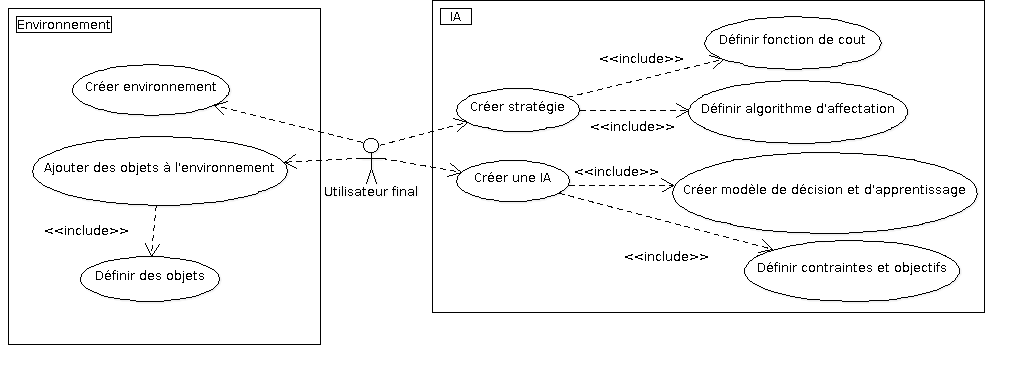
\includegraphics[scale=0.45]{images/uc_main.png}
   \caption{\label{uc_main} Cas d'utilisation généraux}
\end{figure}
\subsection{Ressources}
\begin{figure}[!h]\centering
   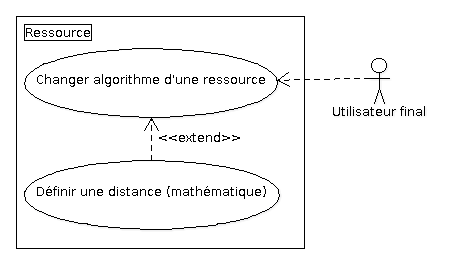
\includegraphics[scale=0.6]{images/uc_ressource.png}
   \caption{\label{uc_main} Cas d'utilisation liés aux ressources}
\end{figure}
\newpage
\subsection{Framework}
\begin{figure}[!h]\centering
   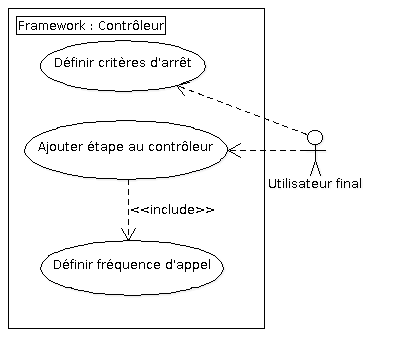
\includegraphics[scale=0.6]{images/uc_framework.png}
   \caption{\label{uc_main} Cas d'utilisation liés au framework}
\end{figure}
\subsection{Partitionnement, Indexation}
\begin{figure}[!h]\centering
   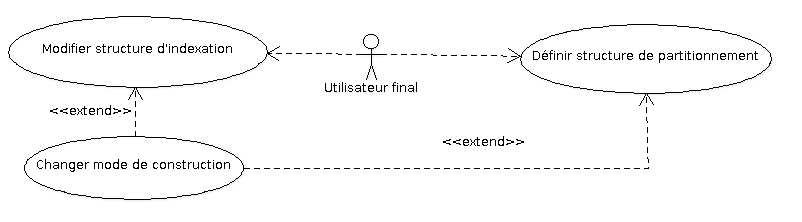
\includegraphics[scale=0.6]{images/uc_index_part.png}
   \caption{\label{uc_main} Cas d'utilisation liés au partitionnement et à l'indexation}
\end{figure}
%
\newpage
\section{Modélisation des entités}

\subsection{Tâche}

Une tâche est définie par une représentation numérique. Ne doit pas être confondue avec l'emplacement de travail (TaskSpot) qui est un objet concret de l'environnement qui peut modifier la  tâche.

\subsection{Contraintes}

Une contrainte est une assertion et sera modélisée sous forme de foncteur renvoyant vrai ou faux.
Il existe plusieurs types de contraintes ayant plusieurs fonctionnements. Chacune possède une priorité qui pourra représenter soit un ordre de traitement par l'IA soit une pénalité lors de l'évaluation. \\

\textbf{Note}~: Il serait intéressant de pouvoirs détecter les contraintes impossibles à tenir en fonction de l'environnement ou tout simplement parce que deux contraintes s'opposent. Le problème de satisfaction de contraintes est à lui tout seul un problème NP-difficile dans la plupart des cas.\\
\indent On supposera durant ce projet que ce point ne pose pas de soucis et que l'utilisateur n'entrera pas des contraintes qui pourront amener le système à se bloquer ou à ne pouvoir satisfaire l'ensemble des contraintes dans un temps raisonnable.\\
\indent Par la suite il pourra néanmoins être intéressant de proposer des algorithmes de déduction de contraintes et de résolution du problème CSP (Constraint satisfaction problem).

\subsubsection{Contraintes de seuils}

Une contrainte de seuil (appliquée à une tâche) est composée d'un opérateur $\leq$ ou $\geq$, et d'une valeur numérique.\\
\indent Ces contraintes possèdent deux fonctions de callback qui doivent se déclencher lorsque l'on franchi le seuil défini, d'un côté et de l'autre (ie, cela implique de garder en mémoire la valeur lors de la vérification précédente).\\
\indent Optionnellement, on peut définir un intervalle de tolérance non nécessairement symétrique.

\subsubsection{Contraintes de de proportionnalité}

Défini une relation de proportionnalité entre 2 ou plusieurs tâches.
On peut imaginer par exemple vouloir 30 \% de pierres contre 70 \% d'or dans le cadre d'un jeu de statégie.\\
\indent Là encore, on peut définir de manière optionnelle un intervalle de tolérance et deux fonctions de rappel qui seront appelées en cas de changement de statut de la contrainte (passage du respect au non respect et inversement).

\subsubsection{Contraintes personnalisées}

Une contrainte personnalisée est une contrainte modélisée par une fonction renvoyant un booléen~: vrai si la condition est vérifiée, faux sinon.
Elles servent à exprimer des contraintes diverses sur les tâches mais aussi sur d'autres éléments de l'environnement en fonction du problème de l'utilisateur.\\

Ces contraintes portent également deux fonctions de rappel pour le changement de statut de la contrainte.

\subsection{Système de contraintes}
Il s'agit d'un système comprenant les tâches ainsi que les contraintes. Les  tâches / contraintes sont potentiellement indépendantes de l'IA qui va résoudre le problème puisqu'elles appartiennent au problème lui même.\\

Ainsi le but du système de contraintes est de centraliser les tâches et les contraintes pour en faciliter l'accès par l'utilisateur et l'IA.\\
\indent Le système pourra également proposer des méthodes de résolution du CSP évoquées plus haut.\\\\

Note~: La description des contraintes peut se faire de manière plus générale et plus souple par l'utilisateur grâce à un design pattern interpréteur (que nous n'implémenterons pas dans l'immédiat).


\subsection{L'environnement}

Il est composé d'un espace au sens mathématique, ainsi que de 3 types d'objets~: les obstacles, les points de travail et les ressources. Il a donc principalement un rôle de conteneur.\\

\'Etant donné que la création de l'environnement peut très vite devenir complexe, un design pattern builder est envisagé, permettant par exemple de charger un fichier d'environnement depuis différents types de fichiers.
Ce sera d'ailleurs le cas pour l'application d'exemple.\\\\

L'environnement est à la fois un observateur et un observable. Il est observé par l'IA et observe les objets dynamiques qu'il contient. Ainsi il s'agit d'un médiateur entre les objets qu'il contient et l'IA.

\subsection{L'espace}

L'espace est simplement défini par un nombre de dimensions et le type de ses coordonnées.
Il contient également les limites de l'espace. L'espace peut donc être imaginé comme un parallélotope droit.

\subsection{Les coordonnées}

Les coordonnées permettent de localiser l'ensemble des objets dans l'espace. Elles présentent deux caractéristiques~: le nombre de composantes et le type de ces composantes. Il s'agit d'un vecteur stockant $n$ composantes d'un type numérique.

\subsection{Les objets}

Les objets évoluent dans l'environnement et plus particulièrement dans l'espace qu'il contient. Ainsi, tous les objets possèdent des coordonnées qui doivent être du même type que ceux de l'espace considéré.\\
\indent Il existe deux types d'objets (pour le moment)~: les objets statiques et les objets dynamiques. Chacun de ces deux types donnent lieu à une hiérarchie d'objets.\\

Tous les objets implémentent une géométrie qui permettra d'effectuer des calculs de collision selon diverses techniques. Par exemple on peut définir un objet par un polygone convexe, un polygone quelconque, un carré, un cercle. Chaque représentation à ses avantages et inconvénients sur les méthodes de collisions~: algorithme du point dans un polygone (convexe), Bounding-Box, rayon de collision, etc.\\

Tous les objets possèdent également une fonction update qui sert à mettre à jour leur état interne régulièrement.

\subsubsection{Les objets statiques}

Il s'agit des objets de l'environnement qui ne peuvent pas bouger. Leur intérêt principal est de définir des obstacles dans l'espace, bloquant le passage aux ressources.\\

\textbf{$\hookrightarrow$ Les obstacles}\\

Il s'agit du seul objet statique concret dont nous avons perçu l’intérêt pour l'instant. Il est là pour modéliser, comme son nom l'indique, un obstacle dans l'espace.

\subsubsection{Les objets dynamiques}

Ce sont des objets qui sont capables d'évoluer.\\

\textbf{$\hookrightarrow$ Les ressources}\\

Elles représentent des objets dont l'IA dispose pour pouvoir les affecter à diverses tâches en vu de satisfaire les contraintes du système de contraintes. Il s'agit encore d'une classe abstraite dont le but est de clarifier l'architecture des objets. On retrouvera différents types de ressources ayant des comportements différents.\\

Ainsi on peut imaginer une ressource qui n'est pas réaffectable lorsqu'elle commence une tâche qui lui est donnée par l'IA, on peut imaginer une ressource qui n'accepte qu'un seul type de tâche, etc. Toutes ses variantes dépendent du problème et seront rajoutées à mesure que le besoin s'en fera sentir.\\
\indent Dans notre cas on n'envisagera qu'une unité simple qui pourra être réaffectée n'importe quand, et une unité qui ne pourra pas être réaffectée.\\\\

Chaque ressource est un agent au sens où il est partiellement autonome. Il évolue indé\-pendamment de l'IA qui ne fait que lui communiquer un ordre (une affectation). C'est la ressource qui se déplace de son propre chef pour se déplacer vers l'objectif. Ainsi chaque ressource possède un algorithme de plus court chemin ainsi qu'une vitesse de déplacement.\\

Comme l'intérêt du partionnement spatial et de l'indexation astucieuse des objets réside dans la diminution du temps de calcul des algorithmes en général, cela implique que les ressources doivent accéder aux structures de partitionnement et d'indexation. Ainsi ce n'est pas l'IA qui s'occupe de stocker ces structures (on peut imaginer dans un jeu vidéo que l'IA soit remplacé par un joueur).\\

\textbf{$\hookrightarrow$ Les emplacements de travail}\\

Ce sont les représentations physiques d'une tâche. C'est à dire des objets qui vont pouvoir modifier une tâche (son \og compteur \fg ) en fonction de certaines conditions.\\
\indent Ainsi, ce sont des observateurs d'une tâche particulière qu'elle notifie en cas de changement.\\

Là encore, on peut imaginer beaucoup de variantes~: des emplacements temporaires – l'emplacement est détruit au bout de tant de temps d'utilisation, des emplacements avec un compteur – l'emplacement se détruit après tant d'utilisation, etc.

\subsection{Les politiques de chevauchement}

Les objets sont paramétrés par une politique de chevauchement~: certains objets peuvent ne pas en chevaucher d'autres.\\
\indent Il s'agit concrètement d'un entier qui permet de définir une priorité sur le chevauchement. Un objet ne peux pas surpasser un objet ayant une valeur plus haute que la sienne.\\
\indent Des constantes sont prévues pour définir des objets \og fantômes \fg ~et des objets que l'on ne peut pas chevaucher, comme les obstacles par exemple.

\subsection{Les fonctions de coûts}

Il existe plusieurs types de fonctions de coûts dont le rôle est similaire : évaluer un objet ou une quantité en fonction de différents paramètres. Classiquement, on peut évaluer la satisfaction d'une contrainte, les paires (ressource / emplacement de travail), la situation globale.\\
La manière dont l'évaluation est faite dépend de la stratégie adoptée.\\

L'implémentation est très libre et souple au vu de ce que le C++ permet de faire, surtout avec le nouveau standard.

\subsection{Les stratégies}

Il s'agit d'une manière de résoudre le problème d'affectation pour satisfaire les contraintes. Elle comporte une manière d'évaluer la situation et un algorithme d'affectation.\\

Une stratégie très simple consiste à ne traiter la satisfaction que d'une contrainte à la fois. Il s'agira de la seule stratégie que nous implémenterons.\\

L'évaluation de la situation est faite en fonction de la stratégie. Voici la stratégie que nous implémenterons (visible également sur le diagramme de séquence du contrôleur de l'IA):
\begin{itemize}
\item Evaluation des contraintes
\item Evaluation des paires ressource / emplacement
\item Evaluation globale des ressources
\item Evaluation de la situation \\
\end{itemize}

Voici un exemple concret des fonctions de coûts associés :
La contrainte $x$ non satisfaite : cette contrainte portait sur la tâche $y$ dont la valeur est trop faible.\\

\begin{itemize}
\item Evaluation de l'intérêt des taskSpots\\
\indent \# Le coût des taskSpots rattachés à $y$ est $1$, sinon $0$.
\item Evaluation d'un individu\\
\indent \# Distance des couples (Indi , TaskSpot)
\item Evaluation globale d'individu\\
\indent \# evalIndi * evalTaskSpot
\item Evaluation situation\\
\indent \# Somme des évaluations globales des individus\\
\end{itemize}

Dans cet exemple très simple on ne veut affecter des ressources qu'aux emplacements susceptibles de faire augmenter la quantité non satisfaite. Ainsi dans l'algorithme d'affectation, les couples (individu, emplacement) où l'emplacement n'est pas rattaché à cette quantité seront nuls et donc ne pourront être choisi.\\\\
L'évaluation de la situation est un indicateur pour l'IA afin qu'elle puisse décider si elle doit changer de stratégie ou non.


\subsection{L'IA}

Il s'agit d'un conteneur de stratégies qui sont organisées selon un modèle (couple d'un modèle de décision et d'observation), pour pouvoir plus facilement traiter le problème d'affectation.

\subsection{Arbres}

Utilisés pour indexer les objets, pour partitionner l'espace. On retrouve beaucoup d'arbres différents ayant chacun leurs avantages et désavantages. En voici une liste assez complète qui pourront être implémentés par la suite~:
\begin{itemize}
\item AtlasGrid
\item R-tree
\item Quadtree
\item Octree
\item BSP
\item KD-tree
\item implicit KD-tree
\item vantage KD-tree
\item R+-Tree
\item R-Tree
\item X-Tree
\item M-Tree
\item Hilbert R-Tree
\item UB-Tree
\end{itemize}

\subsection{Données spatiales}

Etant donné que plusieurs objets qui ne se connaissent pas doivent accéder aux structures de données spatiales (que ce soit la partition de l'espace ou l'index des objets dynamiques), il nous faut une classe dédié à cela.\\
Cet objet possède 3 structures de données qui indexent la structure de l'espace (donc les objets statiques), les tâches et les ressources à partir des conteneurs basiques (des tableaux) de l'environnement.\\

Lors de l'initialisation, le contrôleur créera cet objet automatiquement et passera une référence aux ressources (en passant par l'environnement) et à l'IA.

\subsection{Les algorithmes}
Chaque type d'algorithme définit une hiérarchie de classes héritant toutes d'une classe abstraite définissant l'interface de ce type d'algorithme.\\
On utilisera un design pattern Factory pour permettre une instanciation aisée pour l'utilisateur.

\subsubsection{Algorithmes de plus court chemin}

Les algorithmes de plus court chemin renvoient une liste de noeuds à parcourir pour une ressource pour arriver à son objectif. Il se peut qu'il y ait des déplacements à prévoir au sein d'un noeud mais c'est à la ressource de s'en occuper.

\subsubsection{Algorithmes d'affectation}

Les algorithmes d'affectation prennent en entrée les emplacements de travail 

Etant donné que les algorithmes ne travaillent pas nécessairement sur le même type de données (par exemple la méthode hongroise travaille sur une matrice alors que la recherche du plus proche voisin peut faire appel à des structures d'arbre, etc.), une étape de transformation des données peut avoir lieu.

\section{Architecture du framework}

Cette section s'attele à décrire l'architecture globale du framework~:

\subsection{Contrôleur}

Le contrôleur principal gère le déroulement globale de la simulation. Il s'agit d'une boucle principale avec des critères d'arrêt définis par l'utilisateur (nous proposerons un critère temporel).\\
\indent La boucle principale va effectuer en permanence les même actions, dans le même ordre. Ces actions sont des appels à des contrôleurs locaux ou des actions définis par l'utilisateur parce qu'il en a besoin dans son application~: interception et traitement des entrées claviers, affichage \ldots \\
\indent Par défaut, seules deux actions sont présentes: l'appel au contrôleur local de l'IA et au contrôleur local de l'environnement.\\

Ces actions seront modélisées sous forme d'une liste de fonctions à appeler dans l'ordre. Chaque fonction sera assortie d'un délais d'activation~: toutes les 100ms par exemple.

\subsection{Logger}
Un logger est absolument nécessaire pour un framework afin de repérer le déroulement du flux d'exécution et de localiser d'éventuel(s) problème(s) ou simplement visualiser le processus de calcul. C'est d'ailleurs très utile pour faire des tests unitaires ou d'intégration.\\

\indent Nous mettrons en place un logger sous forme de Design Pattern Chaine de Responsabilité. Chaque maillon de la chaîne sera un logger avec un niveau de log différent (DEBUG, INFO, ERROR \ldots ) et le message transite de maillon en maillon jusqu'à ce que le bon niveau soit atteint.\\
\indent On pourra utiliser une sérialisation dans un fichier texte ou non.\\

Il existera une instance statique du logger pour permettre une utilisation globale. On n'utilisera pas de DP Singleton d'une part parce qu'il est très dur à rendre thread-safe et d'autre part parce pour une raison ou une autre, l'utilisateur final trouvera peut être une utilité à avoir plusieurs loggers.

\subsection{Le modèle multi-thread}
Nous n'implémenterons pas le modèle multithread pour des raisons de temps mais nous le rendrons facilement intégrable, notamment avec la fonction du contrôleur principal. En effet, les actions du contrôleur sont, normalement, toutes indépendantes et peuvent donc être lancées en parallèle.\\

Pour rendre l'application thread-safe à un niveau de granularité plus fin, on utilisera le paramétrage par politique qui permettra de découpler totalement le modèle multi-thread du reste et d'activer / désactiver le support multi-thread à la volée.

\subsection{Les observateurs / observables}
Le design pattern Observateur occupe une place importante notamment lors de la récupération d'information sur l'environnement par l'IA mais également par la notification de mise à jour de plus petites entités au sein de l'environnement (les objets). C'est pourquoi nous avons imaginés deux types de politiques liées à l'observation : une politique active et une politique passive.

\subsubsection{Politique active}

La politique active est le comportement classique lorsque l'on parle du patron Observateur. Dès qu'un changement apparaît sur un observé, il notifie l'observateur qui s'est abonné aux observés.\\
On retrouve ce comportement au niveau du couple Emplacement / Tâche où l'emplacement, sous certaines conditions, va notifier la tâche qui devra se mettre à jour.

\subsubsection{Politique passive}

La politique passive consiste pour l'observé à simplement changer son état indiquant qu'il a changé et préparer le message qui doit être transmis à l'observateur. C'est donc l'observateur qui est actif et va explicitement demander la notification d'état et récuperer les messages des observables qui ont indiqués qu'ils étaient modifiés.\\

Ce comportement apparaît par exemple au niveau de l'observation de l'environnement par l'IA. L'IA va périodiquement choisir de regarder l'état de l'environnement.

\newpage
\section{Diagramme de classes}
\subsection{Algorithmes}
\begin{figure}[!h]\centering
   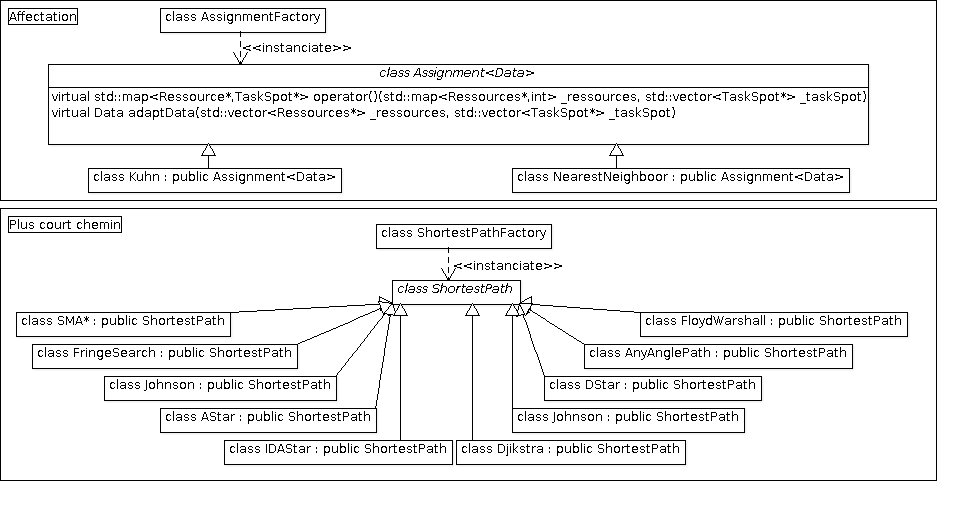
\includegraphics[scale=0.5]{images/c_algo.png}
   \caption{\label{c_algo} Diagramme de classes des algorithmes}
\end{figure}
Pour faciliter l'instanciation des algorithmes de plus court chemin et d'affectation, un Design Pattern Factory est prévu. Il instanciera un objet dérivant de la classe abstraite Assigment ou ShortestPath qui représentent l'interface de manipulation des algorithmes.

\newpage
\subsection{Arbres}
\begin{figure}[!h]\centering %sidewaysfigure
   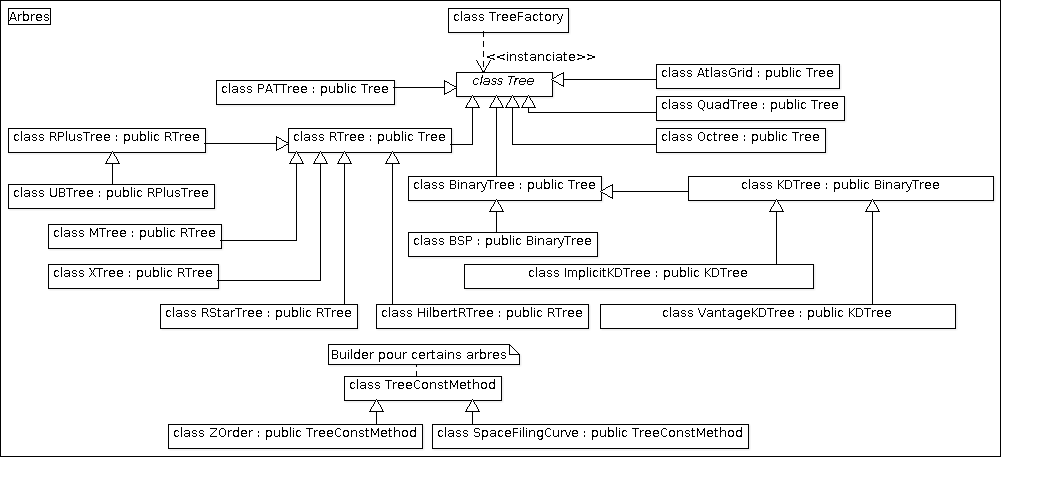
\includegraphics[scale=0.5]{images/c_arbres.png}
   \caption{\label{c_arbre} Diagramme de classes des arbres}
\end{figure}

De la même manière qu'avec les algorithmes, une Factory permettra d'instancier un arbre concret.\\
Certains arbres peuvent se constuire de plusieurs manières, c'est pourquoi on prévoira un Design Pattern Builder pour permettre de monter différemment ces arbres.

\newpage
\subsection{Framework}
\begin{figure}[!h]\centering
   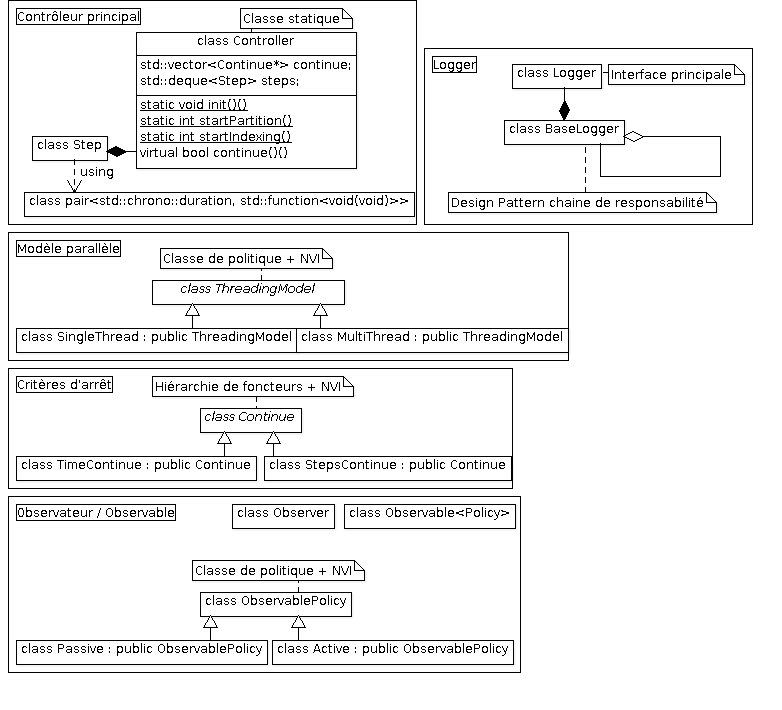
\includegraphics[angle=90, scale=0.6]{images/c_framework.png}
   \caption{\label{c_framework} Diagramme de classes du framework}
\end{figure}

\newpage
\subsection{IA \& Contraintes}
\begin{figure}[!h]\centering
   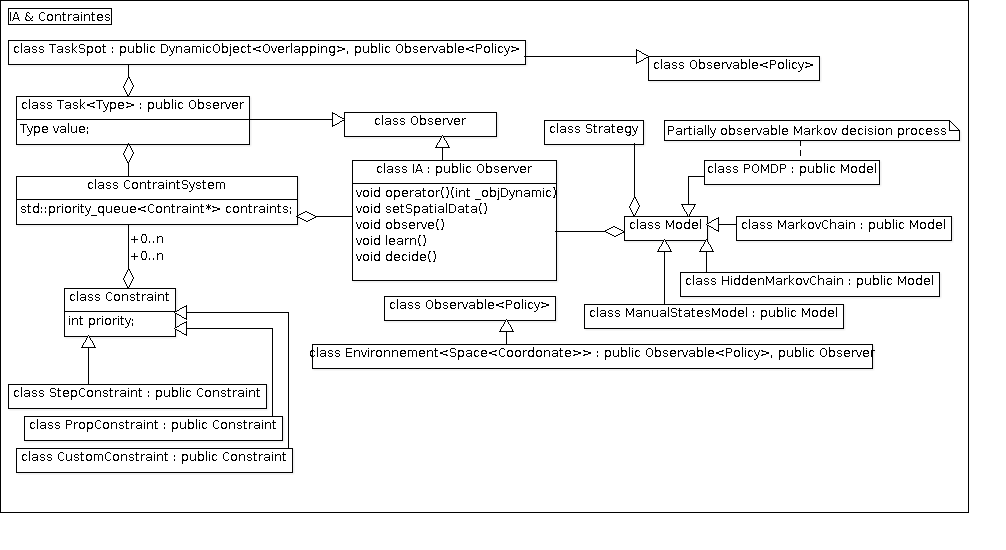
\includegraphics[angle=90, scale=0.5]{images/c_ia_contraintes.png}
   \caption{\label{c_ia_contraintes} Diagramme de classes d'IA et contraintes}
\end{figure}

\newpage
\subsection{{\color{red}Environnement}}}
Une erreur de copié / collé avait fait disparaitre le diagramme de classe du rapport sur la modélisation...
\begin{figure}[!h]\centering
   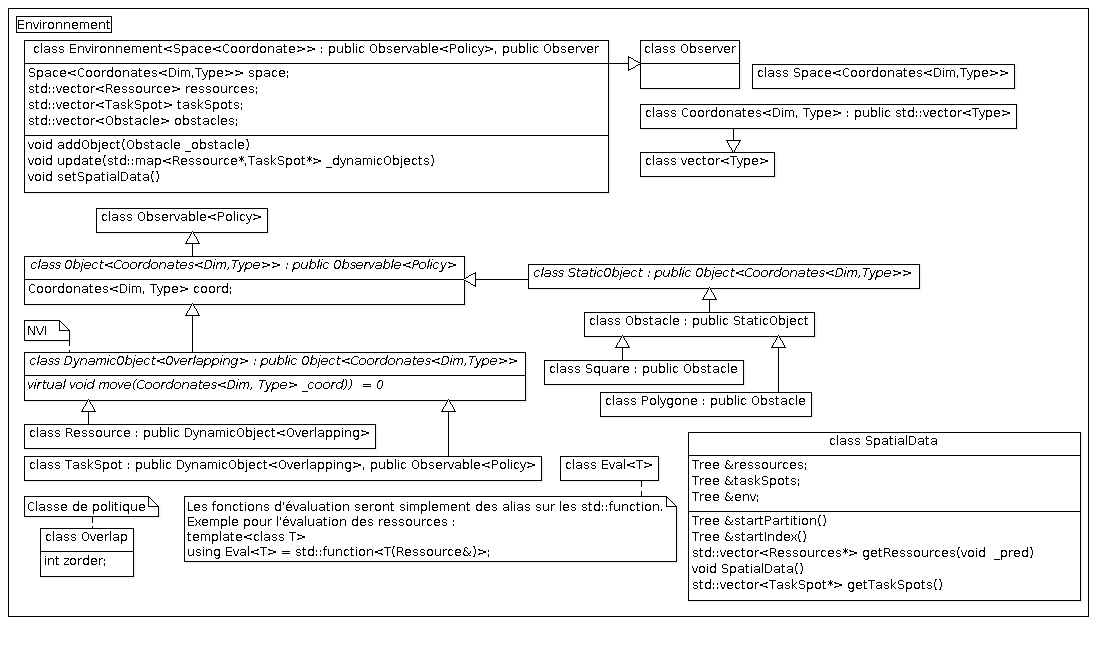
\includegraphics[angle=90, scale=0.5]{images/c_environnement.png}
   \caption{\label{c_ia_contraintes} Diagramme de classes de l'environnement}
\end{figure}

%
\newpage
\section{Scénario et diagrammes de séquences}

On peut distinguer plusieurs scénarios pour notre application. Le scénario utilisateur où l'acteur principal est l'utilisateur final, c'est à dire celui qui va utiliser le framework pour résoudre un problème en fonction de son contexte.\\

Des scénarios annexes existent, relatifs aux sous-systèmes du framework et à l’interaction entre ses composants. Le principal est celui qui intervient durant toute la simulation / résolution et dont l'acteur principal est le contrôleur du framework.

\subsection{Scénario principal}

\renewcommand{\labelitemii}{$\hookrightarrow$}
\renewcommand{\labelitemiii}{$\circ$}
\begin{itemize}
\setlength{\itemsep}{5pt}
\item L'utilisateur définit ses tâches
	\begin{itemize}
	\setlength{\itemsep}{2pt}
	\item Définition des contraintes
	\end{itemize}
\item L'utilisateur définit l'environnement
	\begin{itemize}
	\setlength{\itemsep}{2pt}
	\item Définition de l'espace (dimensions, frontières)
	\item Définition des objets statiques (obstacles)
	\item Définition des objets dynamiques
		\begin{itemize}
		\item Définition des ressources
			\begin{itemize}
			\item Définition d'une fonction de coût
			\end{itemize}
		\item Définition des emplacements de travail
			\begin{itemize}
			\item Observation de l'emplacement par un type de tâche
			\end{itemize}
		\end{itemize}
	\item Paramétrage de l'environnement
		\begin{itemize}
		\item Délais de mise à jour
		\end{itemize}
	\end{itemize}
\item Définition de l'algorithme de partitionnement de l'espace
\item Définition de l'algorithme d'indexation des objets dynamiques	
\item Création des stratégies
	\begin{itemize}
	\setlength{\itemsep}{2pt}
	\item Définition des fonctions d'évaluation
	\item Définition de l'algorithme d'affectation
	\end{itemize}
\item Création de l'IA
\item Définition du modèle de décision et d'observation
\item Ajout des stratégies
\item Paramétrage de l'IA
	\begin{itemize}
	\item Délais entre chaque cycle \og observation – apprentissage – prise de décision - affectation \fg
	\end{itemize}
\item Lancement de la simulation / résolution par le contrôleur du framework.
\end{itemize} %\vspace{4mm}

\newpage
\subsection{Scénarios annexes}

\subsubsection{Initialisation}

L'initialisation est la première étape effectuée lors de l'exécution. Elle se déroule comme suit :\\

	\begin{itemize}
	\setlength{\itemsep}{5pt}
	\item Création de l'objet contenant les données spatiales
	\item Partionnement de l'espace
	\item Indexation : %Listage
		\begin{itemize}
		\item Des ressources
		\item Des emplacements de travail
		\item Des obstacles
		\end{itemize}
    \item Donne un accès en lecture aux données spatiales\\
	\end{itemize}

\begin{figure}[!p]\centering
   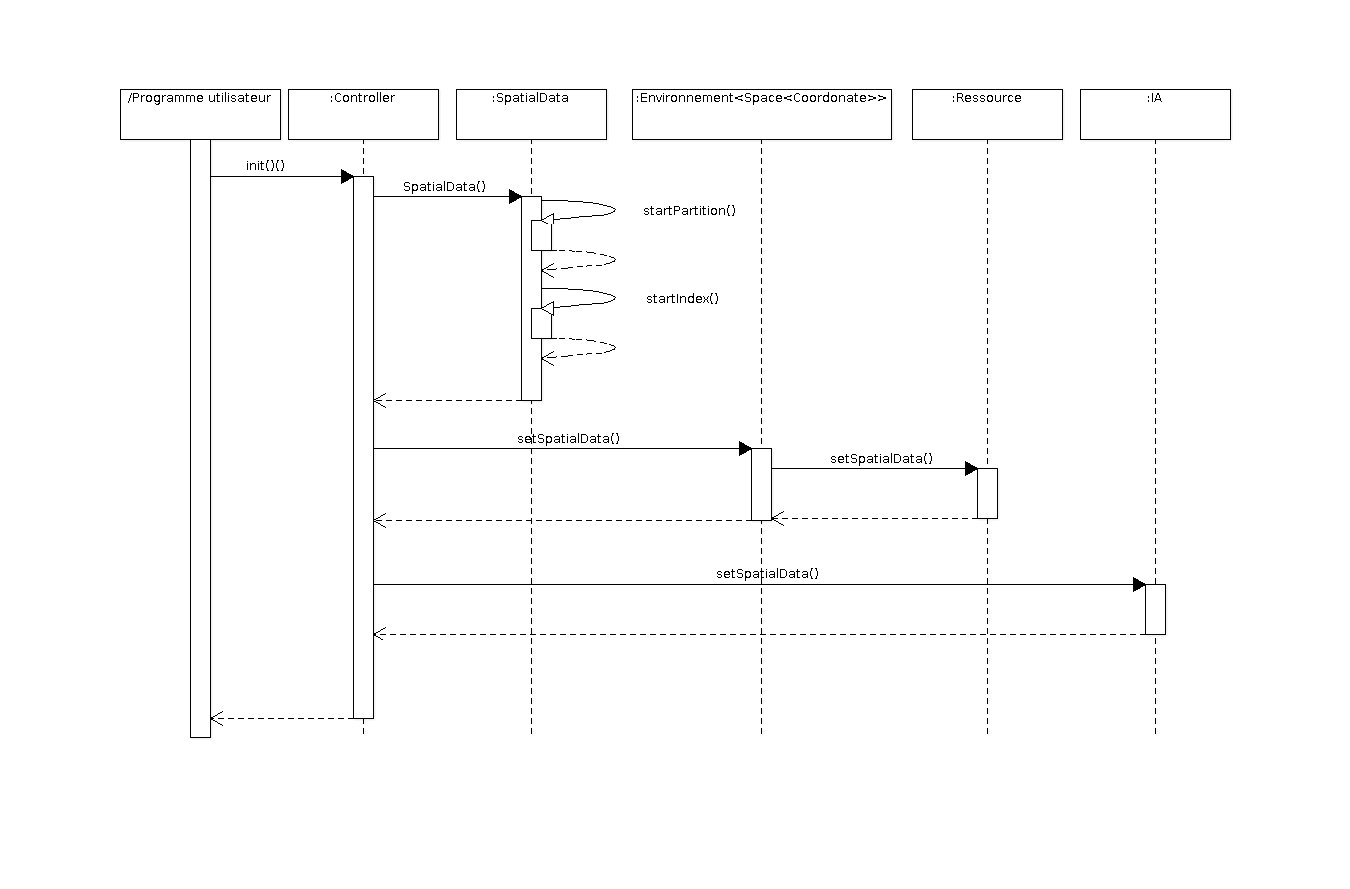
\includegraphics[angle=90, scale=0.5]{images/seq_init.png}
   \caption{\label{seq_init} Séquence d'initialisation}
\end{figure}

(Voir Diagramme de séquence d'initialisation~\ref{seq_init}, page~\pageref{seq_init}).

%
\subsubsection{Contrôleur principal}

	\begin{itemize}
	\setlength{\itemsep}{5pt}
	\item Le contrôleur principal appelle le contrôleur de l'IA si la contrainte de temps est respectée
	\item Le contrôleur de l'IA~:
		\begin{itemize}
		\setlength{\itemsep}{2pt}
		\item Observation du monde par la stratégie courante
		    \begin{itemize}
		    \item Récupération des changements
		    \item Evaluation de la situation
		    \end{itemize}
		\item Apprentissage (non étudié ici)
		\item Prise de décision (non étudié ici - peut être effectué manuellement par l'utilisateur)
		\item Affectation par la stratégie courante
		\item Notification aux ressources des nouvelles affectations
		\end{itemize}
	\item Le contrôleur principal appelle le contrôleur de l'environnement si la contrainte de temps est respectée
	\item Le contrôleur de l'environnement~:
		\begin{itemize}
		\item Mise à jour des ressources
		    \begin{itemize}
		    \item Si pas d'affectation : ne rien faire
		    \item Si affectation : calcul du chemin le plus court
		    \item Si chemin connu : déplacement et calcul de collisions
		    \item ...
		    \end{itemize}
		\end{itemize}
	\item La boucle recommence tant que les conditions sont respectées\\
	\end{itemize}
%
\begin{figure}[!p]\centering
   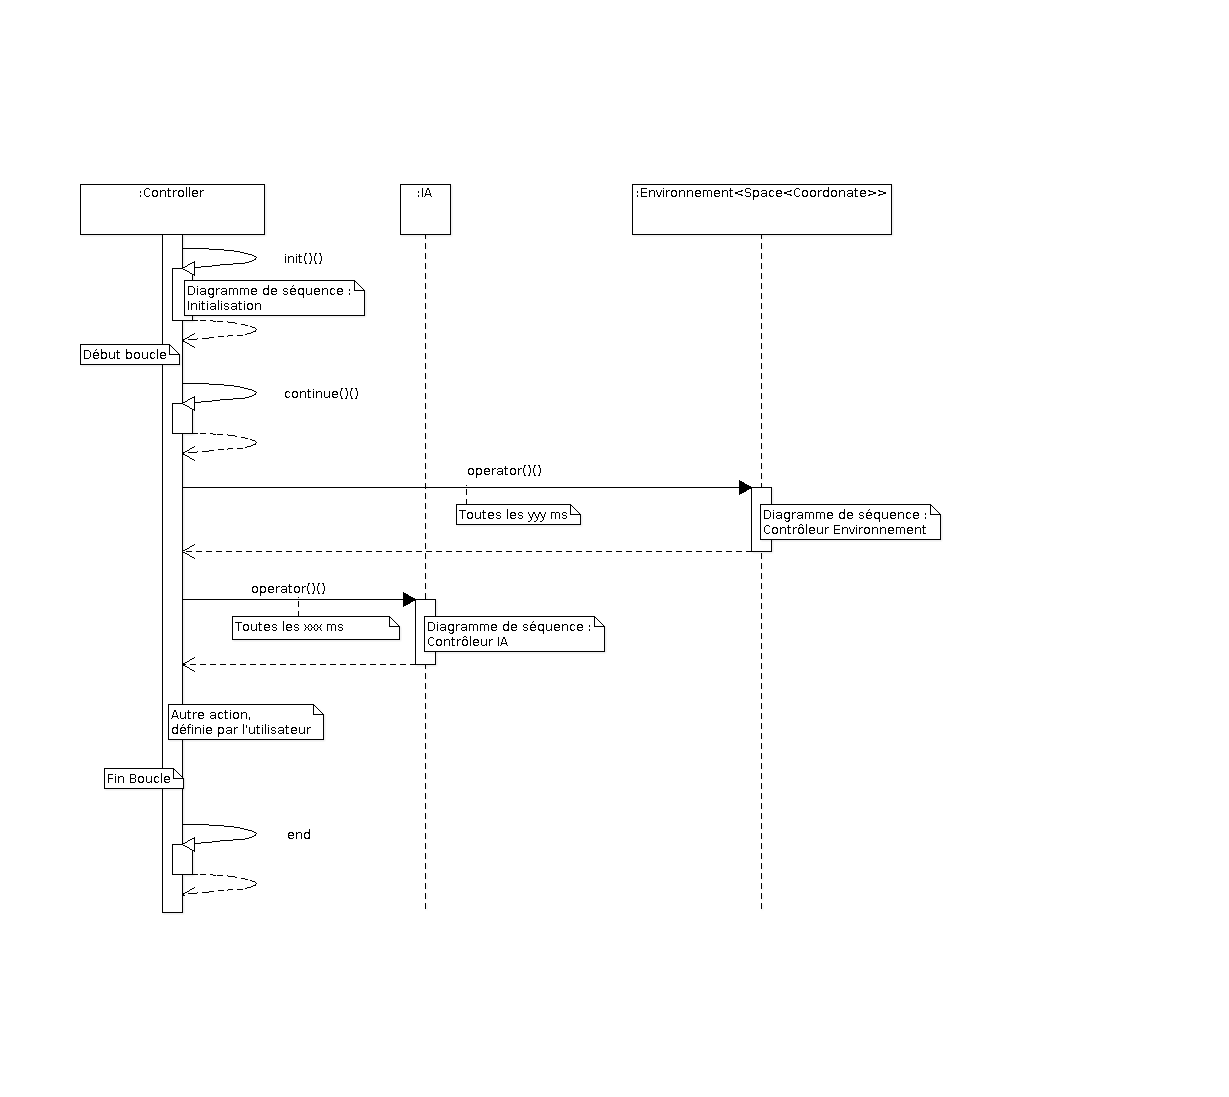
\includegraphics[scale=0.50]{images/seq_simu.png}
   \caption{\label{seq_simu} Séquence de simulation}
\end{figure}

(Voir Diagramme de séquence de simulation~\ref{seq_simu}, page~\pageref{seq_simu}).

\subsubsection{Contrôleur IA}

\begin{figure}[!p]\centering
   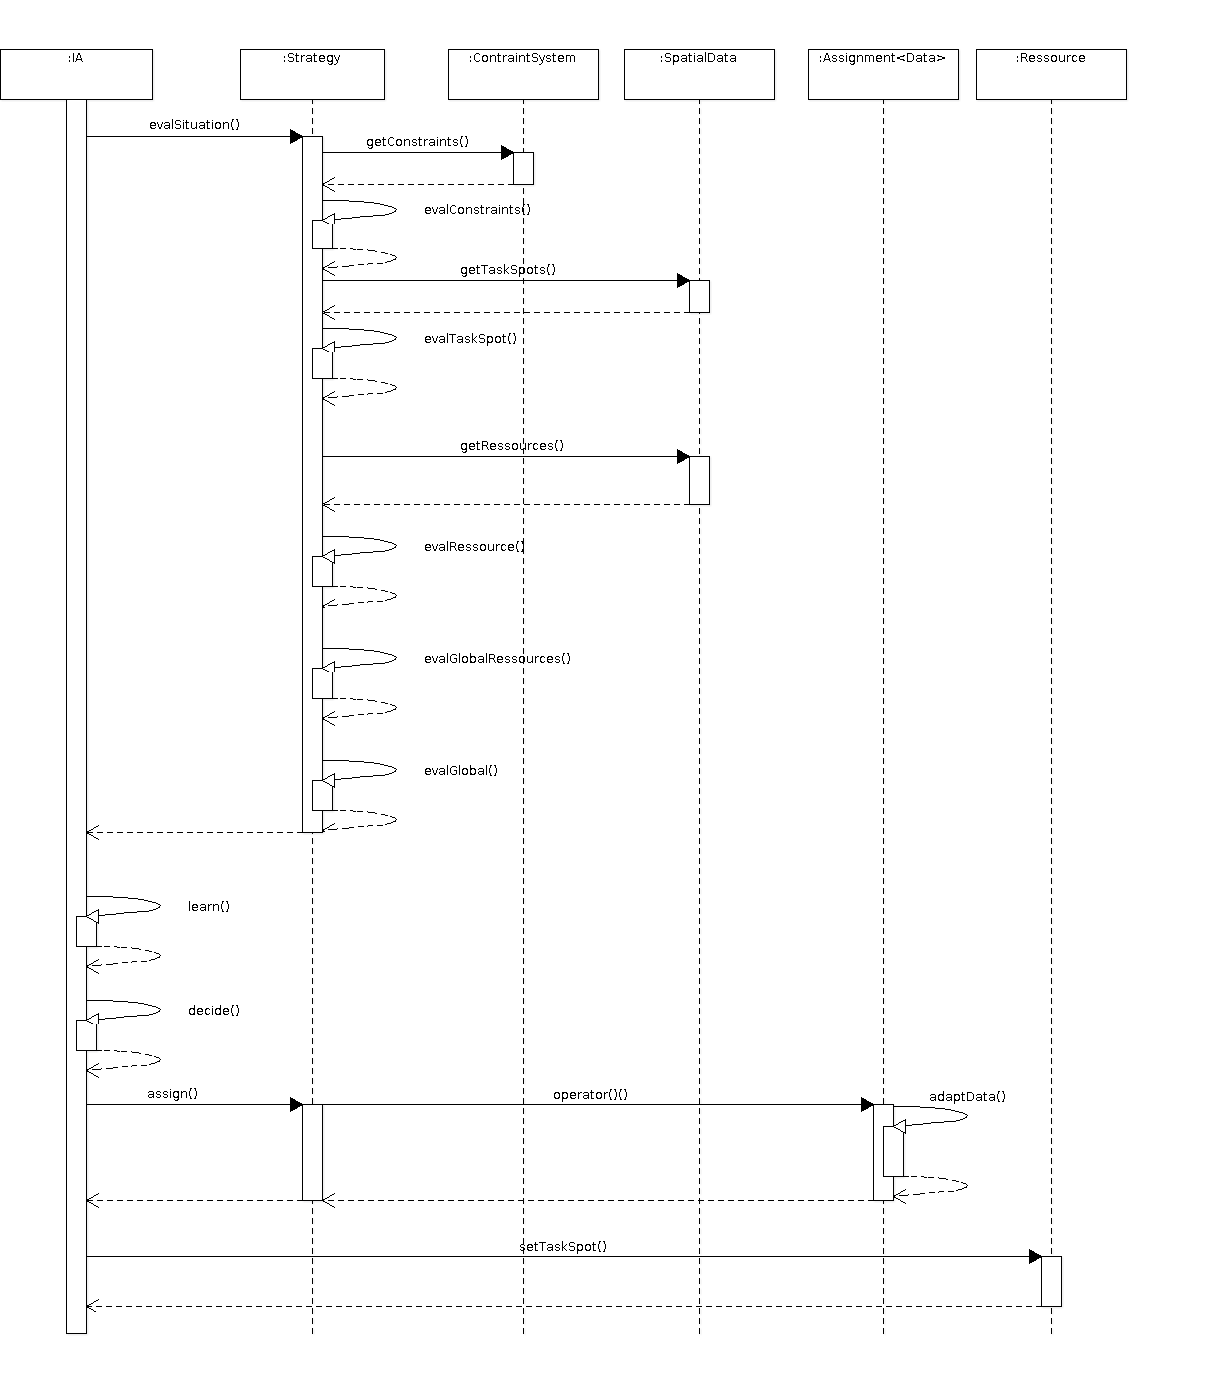
\includegraphics[scale=0.43]{images/seq_ia.png}
   \caption{\label{seq_ia} Séquence du contrôleur de l'IA : cycle \og observation – apprentissage – prise de décision - affectation \fg}
\end{figure}
%
\subsubsection{Contrôleur Environnement}

\begin{figure}[!p]\centering
   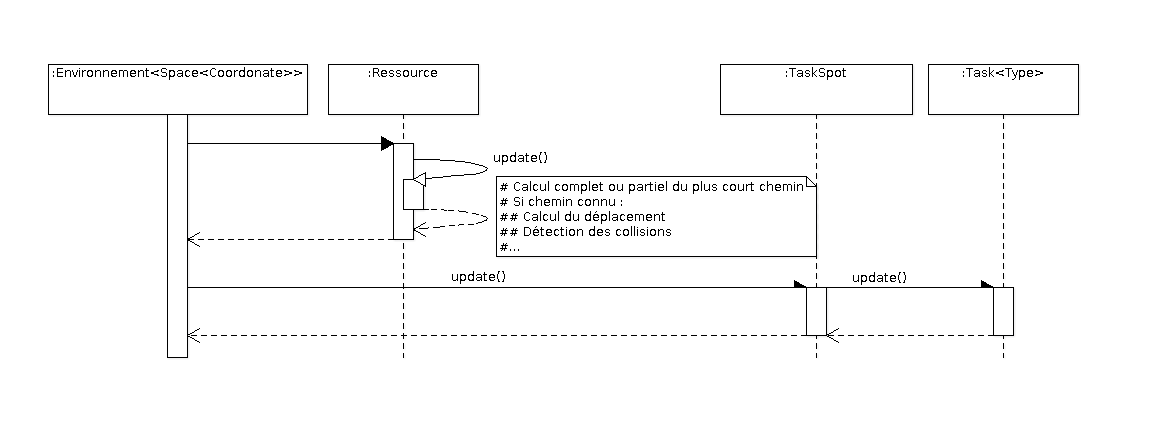
\includegraphics[angle=90, scale=0.55]{images/seq_environnement.png}
   \caption{\label{seq_env} Séquence de mise à jour de l'environnement}
\end{figure}

\newpage
\section{Annexes}

\section{Présentation des pattern récurrents}
\subsection{Idiome NVI}
\subsubsection{Présentation}
L'idiome NVI, pour Non-Virtual Interface, est la réalisation en C++ du design pattern Template Method. Il possède plusieurs avantages notamment dans le développement d'un framework.\\
Il consiste à maintenir la consistance de certains comportements en un point de contrôle du code défini par le développeur. Cela permet d'une inversion de contrôle bénéfique dans de nombreux cas, dont le cas d'un framework puisqu'il déresponsabilise l'utilisateur final de certaines contraintes qui ne pourraient être exprimées que par de la documentation et dont le non respect entraineraient des comportements inattendus difficiles à localiser.\\
NVI est guidé par 4 règles décrites par Herb Sutter dans son article sur la virtualité :
\begin{itemize}
\item Prefer to make interfaces nonvirtual, using Template Method design pattern.
\item Prefer to make virtual functions private.
\item Only if derived classes need to invoke the base implementation of a virtual function, make the virtual function protected.
\item A base class destructor should be either public and virtual, or protected and nonvirtual.
\end{itemize}

\subsubsection{Exemple}
Imaginons une bibliothèque de manipulation de matrices. La bibliothèque propose une classe abstraite Matrice avec l'API globale de toute matrice. On considérera ici la calcul du déterminant. Découle de cette classe une hiérarchie de matrices pour les cas particuliers : matrice triangulaire, matrice diagonale, etc.\\

\begin{figure}[!h]\centering
    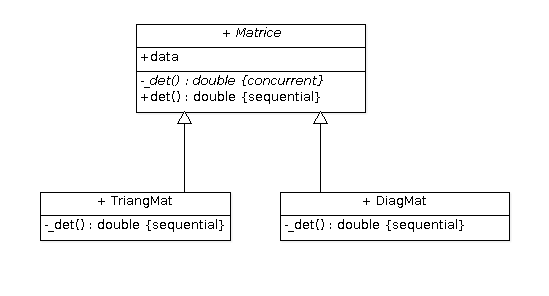
\includegraphics[scale=0.7]{images/nvi_illu.png}
    \caption{\label{nvi_uml} Illustration du NVI.}
\end{figure}

\begin{lstlisting}[label=nvi_code,caption=NVI : principe.,language=C++]
class Matrice
{
public :
    double det() const
    {
        // Pre-traitement : verification d'invariants, lock multithread, etc.
        m.lock();
        assert(data_.check_invariants() == true);
        // Appel de l'implementation
        return _det();
        // Post-traitement
        assert(data_.check_invariants() == true);
        m.unlock();
    }
    
private :
    virtual double _det() const = 0;
    
protected :
    Data data;
    mutex m;
};

class TriangMat : public Matrice
{
private :
    virtual double _det() const 
    {
        // Retourne le produit de la diagonale
    }
}

class DiagMat : public Matrice
{
private :
    virtual double _det() const 
    {
        // Retourne le produit de la diagonale
    }
}
\end{lstlisting}

Ainsi, lorsque l'utilisateur voudra ajouter une nouvelle matrice, disons de forme Hessenberg, il aura simplement à implémenter le calcul du déterminant, les invariants étant toujours vérifiés dans le code de la classe de base qui va appeler l'implémentation.\\
Il y a donc une réelle inversion de contrôle et c'est le développeur du framework qui dirige le client à l'utiliser correctement.\\\\

Nous utiliserons par la suite du projet l'idiome NVI de manière intensive pour permettre de guider le flux d'exécution.

\subsection{Paramétrage par politique}
\subsubsection{Présentation}
Le paramétrage par politique est une technique de programmation développée et démocratisée par Andrei Alexandrescu dans son livre Modern C++ Design: Generic Programming and Design Patterns Applied et dans la bibliothèque Loki dédiée à la méta-programmation en C++ dont beaucoup d'éléments ont été repris dans Boost puis dans le standard 2011.\\\\
Concrètement, il s'agit de profiter de l'héritage multiple et de la métaprogrammation pour permettre de séparer les différents comportements d'une classe ou de plusieurs classes et de créer sur mesure des comportements en combinant plusieurs politiques.

\subsubsection{Fonctionnement}
La clef d'un paramétrage par politique efficace réside dans l'analyse des différents comportements d'une classe ou d'un ensemble de classes. Imaginons que nous ayons à créer une bibliothèque de gestion de graphes. Un graphe peut être représenté sous différentes formes : matrice d'adjacence, matrice d'incidence , ou liste de successeurs. Chaque représentation à ses avantages et ses inconvénients en fonction des applications. On pourrait aisément créer 3 classes différentes mais cela ne serait pas très pertinent. On pourrait simplement templater la classe de graphe mais chaque type donnée n'a pas la même API. De plus, imaginons qu'un graphe puisse être partagé entre plusieurs thread ou non selon les applications.\\
Sans paramétrage par politique, il faudrait un nombre de classes égales au nombre de facteurs multiplié par le nombre de modes par facteur. Cela apporterait évidemment du code redondant et une maintenabilité moindre puisque dans le cas d'un paramétrage par politique on peut isoler complètement un comportement. Pour modifier l'intégralité du modèle multithread d'une application, la modification d'une seule classe de politique est nécessaire.\\\\

Chaque facteur est représenté par une classe abstraite permettant de définir l'API commune à tous les modes et qui pourra être utilisée par les classes paramétrées avec ce facteur. Les classes concrètes implémentent chacun des modes de la politique.\\
Enfin, la classe de services qui doit être paramétrée par politique va être templaté avec chacune des politique et en hériter de manière publique ou privée selon les besoins.

\subsubsection{Exemple}

\begin{figure}[!h]\centering
    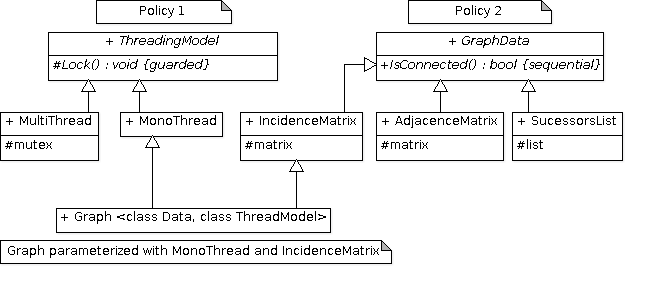
\includegraphics[scale=0.7]{images/policy_illu.png}
    \caption{\label{policy_uml} Illustration du paramétrage par politique.}
\end{figure}

On définit la première hiérarchie de classes correspondant à la première politique :
\begin{lstlisting}[label=policy_1,caption=Définition de la première politique,language=C++]
class ThreadingModel 
{
protected :
    virtual void Lock() = 0;
};

class MultiThread : public ThreadingModel
{
protected :
    virtual void Lock()
    {
        m.lock();
    }
    
    std::mutex m;
};

class MonoThread : public ThreadingModel
{
protected :
    virtual void Lock() = default
};

// ... Autres modeles ...
\end{lstlisting}

On définit la seconde politique :
\begin{lstlisting}[label=policy_2,caption=Définition de la seconde politique,language=C++]
class IncidenceMatrix : public GraphRepresentation
{
public :
    virtual bool IsConnected() const
    {
        // Determine si un graphe est connexe
    }
protected :
    std::vector<std::vector<int>> data;
};

class AdjacenceMatrix : public GraphRepresentation
{
public :
    virtual bool IsConnected() const
    {
        // Determine si un graphe est connexe
    }
protected :
    std::vector<std::vector<bool>> data;
};

//... Autres representations ...
\end{lstlisting}

On définit la classe principale de graphe et on la paramétrise à l'instanciation selon les besoins :
\begin{lstlisting}[label=policy_3,caption=Illustration de la paramétrisation,language=C++]
template <class Rep = AdjacenceMatrix, class ThreadModel = MonoThread>
class Graph : public Rep, public ThreadModel
{
public :
    bool IsConnected() const
    {
        ThreadModel::Lock();
        return Rep::IsConnected();
    }
};

using GraphInciMT = Graph<IncidenceMatrix, MultiThread>;
using GraphAdjMT = Graph<AdjacenceMatrix, MultiThread>;

// Exemples
Graph a; // Adjacence, MonoThread
GraphInciMT b; // Incidence, MultiThread
GraphAdjMT c; // Adjacence, MultiThread

\end{lstlisting}

La classe Graph fait appelle à l'aveugle à sa politique de thread ainsi qu'à sa politique de représentation. La bonne écriture d'une politique est guidée par l'API de la classe abstraite en haut de la hiérarchie mais aucune vérification de type n'est effectuée par la classe Graph. Ainsi, un utilisateur pourrait écrire sa propre politique qui ne serait pas basée sur une des classes abstraites.\\
La partie \verb|using| n'est pas du simple sucre synthaxique puisqu'il contribue également à la maintenabilité de l'application. L'utilisateur final utilise des types en \og{} dur \fg, sans template, ce qui permet, si le besoin s'en fait sentir, de ne changer le template qu'à un unique endroit.

\section{{\color{red}{Notes sur la modélisation}}}

Quelques petites choses ont changé lors de l'implémentation. Notamment, la fabrique pour les algorithmes de plus court chemin a été supprimé puisqu'elle n'avait pas d'intérêt.\\\\

En règle générale, des interfaces, sous la forme de classe abstraite (ie. avec des méthodes virtuelles pures) ont été rajoutées pour la plupart des entitées templatées, afin de pouvoir les manipuler de manière plus générique (et éviter la multiplication des templates dans des classes qui n'en ont pas besoin).\\\\

Les modélisation des chemins, directions et mouvements n'avait pas été faite.

\subsection{Direction}

Une direction est une simple paire comprenant l'indice du vecteur de la base canonique de l'environnement (qui peut être à $n$ dimensions) et un booléen indiquant si le vecteur est dans le sens direct ou indirect.\\
On pourrait imaginer un système plus général où une direction est une combinaison linéaire de vecteurs de la base canonique ce qui permettrait des déplacements autre des déplacements en norme $1$.

\subsection{Mouvement}
Un mouvement représente un vecteur. C'est donc une paire comprenant une direction et sa norme.

\subsection{Chemin}

Il s'agit d'une liste de mouvements. Ils seront parcourus dans l'ordre par une unité qui se déplace tout simplement parce le chemin calculé peut dépendre de l'ordre des mouvements (peut être qu'un autre ordre de parcours poserait problème à cause d'obstacles).


